\section{Simplified ByteNet}

The implementation of the ByteNet model spends $37\%$ of its time waiting for data transfer between GPU and CPU and even more time waiting on the TensorFlow service. This is because of the large amount of weights and operations that is used in the ByteNet model.

To solve this issue a simplified version of ByteNet has been created. This uses less weights and less operations than ByteNet, but remain true to principals behind ByteNet. Those principals is running in linear time, parallelize over both sequence and observations, have be resolution persistent meaning that the size of the encoded representation scales with the sequence length. The simplified version also maintains the bottleneck of 200 dimensions that ByteNet has in its dilated-convolution layer.

The idea behind this is simple, if the initial embedding dimensionality is set to 200 then the compression and decompression layers that exists before and after the dilated convolution are not needed. Of cause these layers adds non-linearities and weights to the model, thus one should not expect the model to perform equally well. Instead the model should before almost as well and be significantly faster.

\begin{figure}[H]
    \centering
    \begin{subfigure}[b]{0.45\textwidth}
        \centering
        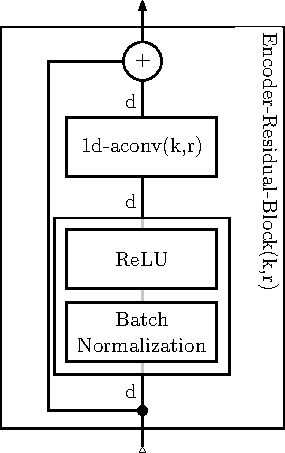
\includegraphics[scale=1]{theory/bytenet-small-residual-block.pdf}
        \caption{Residual Block used in encoder.}
    \end{subfigure}
    ~ %
    \begin{subfigure}[b]{0.45\textwidth}
        \centering
        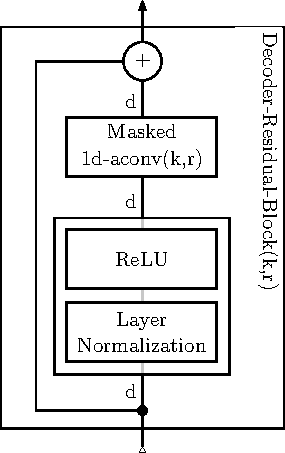
\includegraphics[scale=1]{theory/bytenet-small-residual-block-causal.pdf}
        \caption{Residual Block used in decoder.}
    \end{subfigure}
    \caption{The residual blocks used in the Simplified ByteNet model. The blocks are denoted by Encoder-Residual-Block$(k,r)$ and Decoder-Residual-Block$(k,r)$, where $k$ is the kernel width and $r$ is the dilation rate.}
    \label{fig:result:simple-bytenet:residual-block}
\end{figure}

In terms of weights the simplified ByteNet model has approximately $\sfrac{5}{9}$ times less weights than the ByteNet model. The simplified ByteNet model also has approximately one third of the operations as the ByteNet model. Based on these parameters one should expect less transfer time and less time spend waiting for the TensorFlow service.

The simplified ByteNet model was validated identically to the how the ByteNet model was validated. The results (appendix \ref{appendix:result:bytenet-small}) where very similar with some minor differences. Memorizing WMT NewsTest took fewer iterations, this is likely because there are fewer parameters. The simplified ByteNet model learned the synthetic digits problem better, with a misclassification error of $0.25$. An explanation could for the improved misclassification error is that the the simplified ByteNet model has fewer parameters and non-linear transformation, this might make it overfits less.

\subsection{Performance Profiling}

To compare the performance of the simplified ByteNet model with the normal ByteNet model, the performance experiment from the normal ByteNet model was repeated using the simplified ByteNet model. This experiment learns the WMT NewsTest dataset over 300 epochs. Both a 1 GPU and a 4 GPU setup was used in the experiments.

\begin{figure}[h]
    \centering
    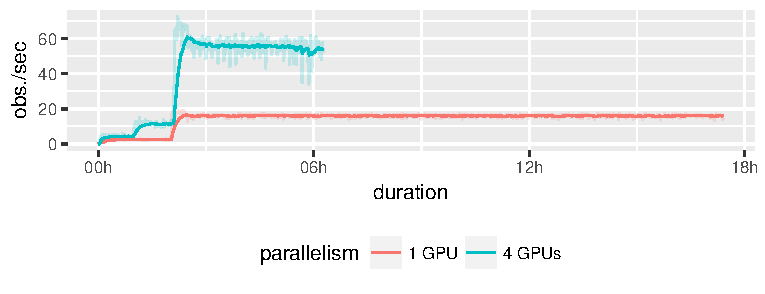
\includegraphics[scale=1]{bytenet-small/timing-gpus.pdf}
    \caption{Comparing observations per second, depending on the number of GPUs used.}
    \label{fig:result:simple-bytenet:timing-gpus}
\end{figure}

Measuring the total time spend and the observations per second as seen in figure \ref{fig:result:simple-bytenet:timing-gpus} reveals that the simplified ByteNet model is faster. On 1 GPU the simplified ByteNet model is about $20\%$ faster. This is quite far from the best case $66\%$, that one would get from reducing the number of operation to $\sfrac{1}{3}$.

On 1 GPU there is no data transfer, thus it is only the TensorFlow service and the computation that takes time. Assuming the actual computation time is not the most time consuming part, reducing the number of operations to $\sfrac{1}{3}$ should result in a $\sfrac{2}{3}$ computational performance gain. This is of cause an approximation as there is still the embedding layer, the concatenation of encoding and decoding, and the final output layer, thus $\sfrac{2}{3}$ the operations is an upper bound.

Comparing the time spend in the 1 GPU experiment and the 4 GPU experiment, and because very little data transfer happens when using 1 GPU. The data shows that approximately $40\%$ time is spend transferring data. This is approximately the same as the $37\%$ in the normal ByteNet model. The number of weights is reduced by $\sfrac{5}{9}$, thus one would expect the transfer time to be reduced by this order, however that is not the case.

\begin{figure}[h]
    \centering
    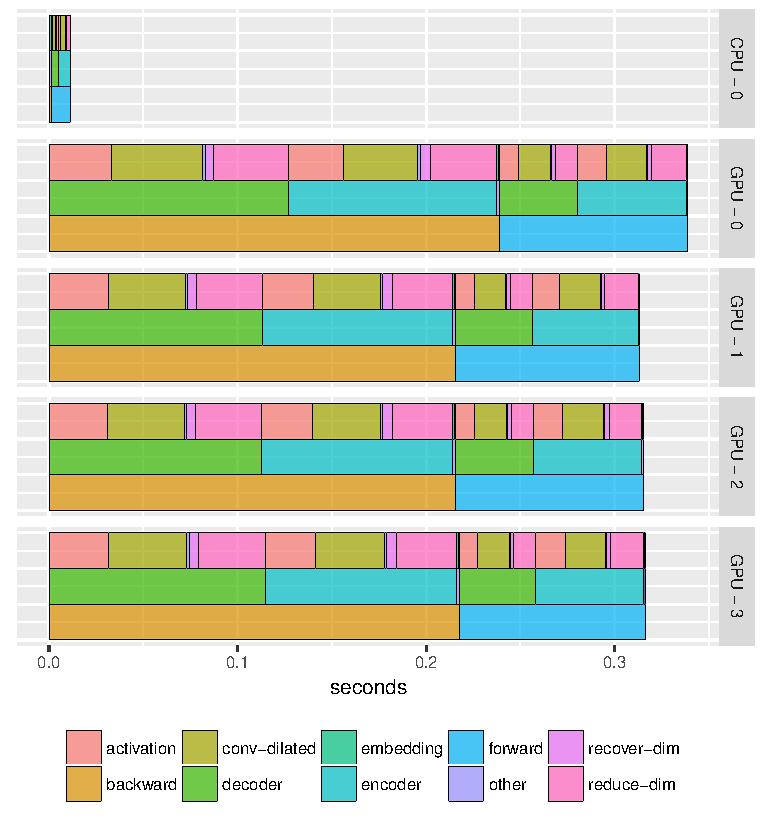
\includegraphics[scale=1]{bytenet-small/profile-grouped-gpu4.pdf}
    \caption{Shows time spend executing operations in each part of the ByteNet model, this excludes the waiting time. Each part exists in a hierarchy, which is visualized as levels. The bottom level is the least detailed level, it just splits the model in the backward and forward pass. The next level, splits the model in the encoder and decoder. The last level at the top, primarily splits the Simplified ByteNet Residual Blocks.}
    \label{fig:result:simple-bytenet:profile-grouped}
\end{figure}

Finally the TensorFlow profiler can be used to investigate what takes time. When processed the results are similar to those from the normal ByteNet model, see figure \ref{fig:result:simple-bytenet:profile-grouped}.

From figure \ref{fig:result:simple-bytenet:profile-grouped} that much of the time is spend in the \textit{activation layer}. The \textit{activation layer} is the layer that contains the normalization and ReLU operation. This validates the idea that it is the number of operations and not the operations themselves that cost in terms of time. The dilated convolution (called \textit{conv-dilated}) is a much more complex operation than normalization or ReLU, but TensorFlow implements it using just a few operations, thus it doesn't consume that much time. As mentioned earlier the TensorFlow team is aware of this performance issue, and tries to solve it my automatically compiling GPGPU (CUDA or OpenCL) kernels that combines multiple operations into one, but this is still very experimental and doesn't yet provide a performance when using multiple GPUs \cite{citation-needed}.

\clearpage
\subsection{WMT Translation Task}

\todo[inline]{Given the minor performance gain both in computation and data transfer, the Simplified ByteNet model is not really worth it.}
